\documentclass[11pt]{article}
\usepackage[letterpaper,landscape,margin=1.4cm]{geometry}
\usepackage{graphicx}
\usepackage{enumitem}
\usepackage{xcolor}
\usepackage{microtype}
\usepackage[hidelinks]{hyperref}

\setlist{nosep, leftmargin=1.6em}
\setlength{\parindent}{0pt}
\setlength{\parskip}{0.3em}
\pagestyle{empty}
\newcommand{\code}[1]{\texttt{#1}}
\newcommand{\wire}[2]{\textcolor{#1}{\rule[0.25ex]{1.6em}{1.6pt}}\,\textbf{#2}}
\definecolor{wred}{RGB}{220,20,20}
\definecolor{wwhite}{RGB}{170,170,170}
\definecolor{wgreen}{RGB}{10,170,50}
\definecolor{worange}{RGB}{250,140,0}
\definecolor{wyellow}{RGB}{220,190,0}
\definecolor{wblue}{RGB}{30,90,250}
\definecolor{wgrey}{RGB}{154,160,166}
\definecolor{hOrange}{HTML}{EE8A5C}
\definecolor{hPurple}{HTML}{5A2F8C}
\definecolor{hBrown}{HTML}{5B4038}
\definecolor{hBlack}{HTML}{25211F}
\definecolor{hYellow}{HTML}{E8CF2A}
\definecolor{hTeal}{HTML}{1F7A68}

\begin{document}

{\Large\bfseries H723 power measurement --- the bench as drawn for the paper}\hfill{\small 2 November 2026, revision 3}

\smallskip
{\small \textbf{Nothing is cut, nothing is bought, and every cable is a standard USB cable.} The spare F411 Black Pill is
the USB breakout and the logger at once; the debugger stays wired, in its harness's own colours.}

\begin{center}
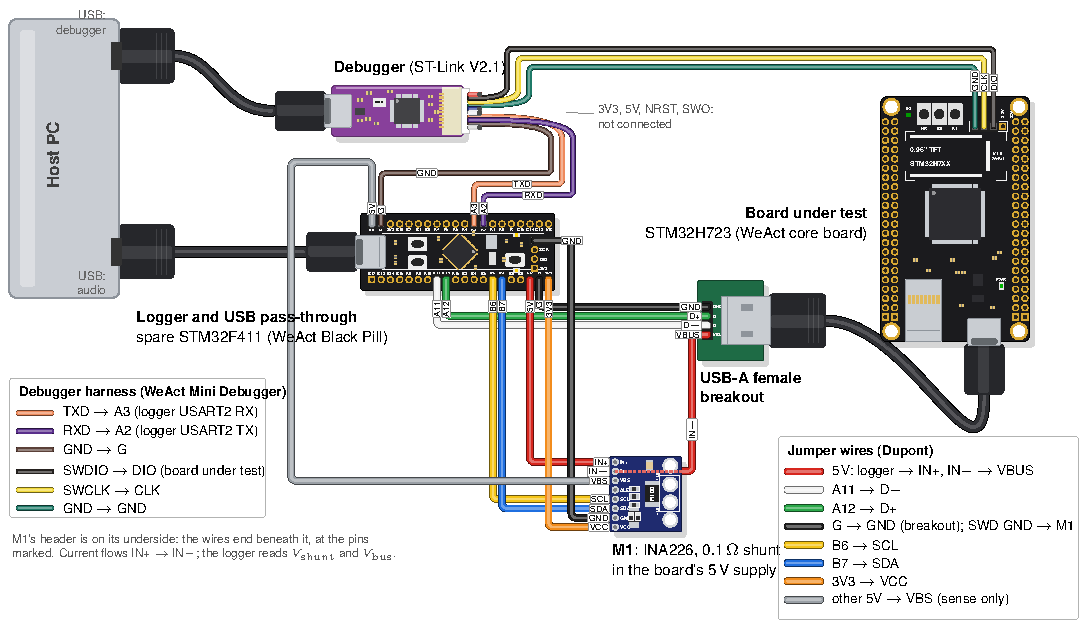
\includegraphics[width=\linewidth,height=0.62\textheight,keepaspectratio]{figures/power-bench-h723.pdf}
\end{center}

\vspace{-0.8em}
{\small
\begin{minipage}[t]{0.5\linewidth}
\textbf{Connect it in this order}
\begin{enumerate}
\item A \textbf{standard USB-A to USB-C cable} from the laptop into the spare F411.
\item \wire{wred}{5V}: spare F411 \code{5V} $\to$ M1 \code{IN+}; M1 \code{IN$-$} $\to$ breakout \code{VBUS}.
\item \wire{wwhite}{A11$\to$D$-$}, \wire{wgreen}{A12$\to$D+}, \wire{black}{G$\to$GND}: spare F411 to your breakout.
\item \wire{wyellow}{B6$\to$SCL}, \wire{wblue}{B7$\to$SDA}, \wire{worange}{3V3$\to$VCC}, \wire{black}{GND$\to$GND}
(its 4-pin end header), \wire{wgrey}{other 5V$\to$VBS}: spare F411 to M1. All of M1's pins are on its one header.
\end{enumerate}
\end{minipage}\hfill
\begin{minipage}[t]{0.47\linewidth}
\phantom{\textbf{x}}
\begin{enumerate}[start=5]
\item Debugger: \wire{hOrange}{TXD$\to$A3}, \wire{hPurple}{RXD$\to$A2}, \wire{hBrown}{GND$\to$G} on the spare F411;
\wire{hBlack}{SWDIO$\to$DIO}, \wire{hYellow}{SWCLK$\to$CLK}, \wire{hTeal}{GND$\to$GND} on the H723. Its red (3V3) and
light-grey (5V) wires stay loose: \textbf{black is SWDIO here, not ground}.
\item The H723's usual cable into the breakout. Checks: \code{dmesg -w} silent with the spare F411 alone; flash script
zeroes \code{DBGMCU\_CR}; one idle reading after a scripted flash equals one after replugging the cable.
\end{enumerate}
\end{minipage}}

\vfill
{\scriptsize\color{black!60} Drawn to scale from the parts' own drawings by \code{docs/figures/power-bench-h723.tex}
(shared parts in \code{bench-parts.tex}); the INA226 module is drawn from a photo of the one on the bench; only the USB-A breakout is still generic, until checked against
the bench. The other boards: \code{power-wiring-boards.pdf}.}

\end{document}
